\documentclass[crop, tikz]{standalone}
\RequirePackage{luatex85}

\usepackage{fontawesome}
\usepackage{fontspec}
\usetikzlibrary{
    backgrounds,
    patterns,
    mindmap,
    shapes,
    shapes.misc,
    fit,
    trees,
    tikzmark,
    arrows,
    arrows.meta,
    positioning,
    decorations.pathmorphing,
    shapes.geometric,
    decorations.pathreplacing
}

\newfontfamily{\ttfamily}{Fira Code}
\usepackage{fontspec}
\setmainfont{Liberation Sans}
\newfontfamily\ExtraLight{Liberation Sans}
\newfontfamily\Light{Liberation Sans}
\newfontfamily\Book{Liberation Sans}
\newfontfamily\Medium{Liberation Sans}

\definecolor{greenGood}{HTML}{99FF99}
\definecolor{redBad}{HTML}{FF9980}

\makeatletter
\tikzset{rum-node/.style={draw,circle,fill=white,minimum width=2cm}}
\tikzset{>=latex}

\makeatother

\begin{document}
    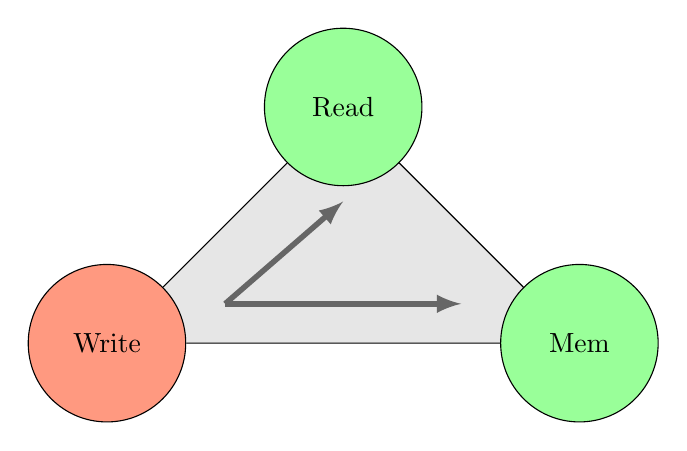
\begin{tikzpicture}[]
        \node [rum-node, fill=greenGood] (memory) at ( 3, 0) {Mem};
        \node [rum-node, fill=redBad] (write) at (-3, 0) {Write};
        \node [rum-node, fill=greenGood] (read) at ( 0, 3) {Read};
        \draw (read) -- (write) -- (memory) -- (read);
        \begin{scope}[on background layer]
            \fill [gray, opacity=0.2]
                (read.center) --
                (write.center) --
                (memory.center) -- cycle;
        \end{scope}

        \coordinate[below=1.2 of read.center] (change-read);
        \coordinate[above=0.5 of memory.center] (change-memory);
        \coordinate[left=1.5 of change-memory] (change-memory-angle);
        %\coordinate[right=2.5 of change-pointer] (change-angle);
        \coordinate[above=0.5 of write.center] (change-anchor);
        \coordinate[right=1.5 of change-anchor] (change-start);
        \draw[->, line width=2pt, color=black!60] (change-start) -- (change-read);
        \draw[->, line width=2pt, color=black!60] (change-start) -- (change-memory-angle);

    \end{tikzpicture}
\end{document}
